
\documentclass[12pt]{article}

% --- Preamble ---
\usepackage[utf8]{inputenc}
\usepackage[T1]{fontenc}
\usepackage{amsmath, amssymb, amsfonts, amsthm}
\usepackage{physics} % For \pdv, \grad, \vb, etc.
\usepackage{tikz}
\usetikzlibrary{calc, positioning, arrows.meta}
\usepackage{xcolor}
\usepackage{geometry}
\geometry{margin=1in}

\title{Vertex Model Master Derivations: Hessian and Shear Modulus}
\author{Gemini CLI | Expert Computational Biophysicist}
\date{\today}

\begin{document}

\maketitle

\section{Introduction}
This document provides the definitive mathematical reconciliation between standard literature (Merkel \& Manning 2018) and the analytical derivations in \texttt{vm\_human\_calculations}. It serves as the canonical reference for implementing the Hessian matrix ($\mathcal{H}$) and the macroscopic shear modulus ($g$) under Lees-Edwards Boundary Conditions (LEBC).

\section{Definitions \& State Variables}

The energy functional $E$ for a tissue of $N_c$ cells is defined as:
\begin{equation}
    E = \sum_{\alpha=1}^{N_c} \left[ \frac{K_A}{2}(A_\alpha - A_0)^2 + \frac{K_P}{2}(P_\alpha - P_0)^2 \right]
\end{equation}

\subsection{Conjugate Variables (Stress Coefficients)}
To facilitate higher-order derivatives, we define the following coefficients:
\begin{itemize}
    \item \textbf{Cell Pressure:} $\Pi_\alpha = -\pdv{E}{A_\alpha} = -K_A(A_\alpha - A_0)$
    \item \textbf{Edge Tension:} $T_\alpha = \pdv{E}{P_\alpha} = K_P(P_\alpha - P_0)$
\end{itemize}

\subsection{Physical Distance and LEBC Unwrapping}
Under simple shear strain $\gamma$, the physical distance $\Delta \vb{r}_{ij}$ must be unwrapped to account for the periodic image shift. For a box of dimensions $(L_x, L_y)$:
\begin{align}
    n_y &= \text{round}\left(\frac{y_j - y_i}{L_y}\right) \\
    \Delta y &= (y_j - y_i) - n_y L_y \\
    \Delta x &= (x_j - x_i) - n_y(\gamma L_y) - L_x \cdot \text{round}\left(\frac{(x_j - x_i) - n_y(\gamma L_y)}{L_x}\right)
\end{align}

\section{First Derivatives (Forces)}

The force on vertex $i$ is $\vb{f}_i = -\pdv{E}{\vb{r}_i}$.
\begin{equation}
    \pdv{E}{\vb{r}_i} = \sum_{\alpha \in \text{cells}(i)} \left[ -\Pi_\alpha \grad_i A_\alpha + T_\alpha \grad_i P_\alpha \right]
\end{equation}

\subsection{Geometric Gradients}
\begin{itemize}
    \item \textbf{Area Gradient:} $\grad_i A_\alpha = \frac{1}{2} \hat{\vb{z}} \times (\vb{r}_{i+1} - \vb{r}_{i-1}) = \frac{1}{2} (y_{i+1} - y_{i-1}, x_{i-1} - x_{i+1})^T$.
    \item \textbf{Perimeter Gradient:} $\grad_i P_\alpha = \sum_{j \in \text{neigh}(i)} \hat{\vb{t}}_{ij}$, where $\hat{\vb{t}}_{ij} = \frac{\vb{r}_i - \vb{r}_j}{|\vb{r}_i - \vb{r}_j|}$ is the unit vector pointing \textit{away} from neighbor $j$ toward vertex $i$.
\end{itemize}

\section{The Hessian Matrix ($\mathcal{H}$)}

The Hessian $H_{ij}^{\mu\nu} = \pdv{E}{r_i^\mu}{r_j^\nu}$ is rigorously separated into \textbf{Modulus (Stiffness)} and \textbf{Stress (Geometric)} components.
\begin{equation}
    \mathcal{H}_{ij} = \mathcal{H}_{ij}^{\text{Mod}} + \mathcal{H}_{ij}^{\text{Stress}}
\end{equation}

\subsection{Modulus Terms}
\begin{equation}
    \mathcal{H}_{ij}^{\text{Mod}} = \sum_\alpha \left[ K_A (\grad_i A_\alpha \otimes \grad_j A_\alpha) + K_P (\grad_i P_\alpha \otimes \grad_j P_\alpha) \right]
\end{equation}

\subsection{Stress Terms}
\begin{equation}
    \mathcal{H}_{ij}^{\text{Stress}} = \sum_\alpha \left[ -\Pi_\alpha \grad_i \grad_j A_\alpha + T_\alpha \grad_i \grad_j P_\alpha \right]
\end{equation}

\begin{itemize}
    \item \textbf{Area Stress:} For $j = i+1$, $\grad_i \grad_{i+1} A_\alpha = \frac{1}{2} \begin{pmatrix} 0 & 1 \\ -1 & 0 \end{pmatrix}$.
    \item \textbf{Perimeter Stress:} For connected vertices $i \neq j$, $\grad_i \grad_j P_\alpha = -\frac{1}{l_{ij}} (\vb{I} - \hat{\vb{t}}_{ij} \otimes \hat{\vb{t}}_{ij})$.
\end{itemize}

\section{Strain Derivatives under LEBC}

Calculating the shear modulus requires first and second total derivatives of the energy with respect to the shear strain $\gamma$. In a periodic box $(L_x, L_y)$, the Lees-Edwards boundary condition (LEBC) introduces specific $\gamma$-dependencies through the unwrapping shift.

\subsection{Area Strain Derivatives}
Contrary to standard affine transformations where $\det \mathbf{\Lambda} = 1$ implies area invariance, the \textit{unwrapped} area of a cell crossing the $y$-boundary under LEBC has a non-zero first derivative:
\begin{equation}
    \pdv{A_\alpha}{\gamma} = L_y \left[ \bar{y}_e^{(L\alpha)} - \bar{y}_e^{(R\alpha)} \right]
\end{equation}
where $\bar{y}_e^{(L\alpha)}$ and $\bar{y}_e^{(R\alpha)}$ are the average $y$-coordinates of the vertices on the left and right edges that cross the periodic boundary. The second derivative is zero: $\pdv[2]{A_\alpha}{\gamma} = 0$.

\subsection{Perimeter Strain Derivatives}
The first derivative represents the projection of the horizontal shear displacement onto the edge axis:
\begin{equation}
    \pdv{P_\alpha}{\gamma} = \sum_{e \in \text{crossing}(\alpha)} \xi(\vb{l}_e) L_y \frac{\vb{l}_e \cdot \hat{\vb{x}}}{l_e} = \sum_{e \in \text{crossing}(\alpha)} \xi(\vb{l}_e) L_y \cos\theta_e
\end{equation}
where $\xi(\vb{l}_e) = \pm 1$ accounts for the orientation of the crossing edge relative to the boundary traversal (CCW).

The second derivative captures the curvature of the edge length under shear:
\begin{equation}
    \pdv[2]{P_\alpha}{\gamma} = \sum_{e \in \text{crossing}(\alpha)} L_y^2 \frac{\sin^2\theta_e}{l_e}
\end{equation}
where $\theta_e$ is the angle between the crossing edge and the $x$-axis.

\section{The Affine Force Vector ($\vb{\Xi}$)}
The vector $\mathbf{\Xi}_i^\mu = \pdv{E}{r_i^\mu}{\gamma}$ represents the forces generated on vertices by an infinitesimal affine box shear. It involves mixed derivatives:
\begin{equation}
    \mathbf{\Xi}_i^\mu = \sum_{\alpha \in \text{cells}(i)} \left[ K_A \pdv{A_\alpha}{\gamma} \pdv{A_\alpha}{r_i^\mu} + K_P \pdv{P_\alpha}{\gamma} \pdv{P_\alpha}{r_i^\mu} - \Pi_\alpha \pdv{A_\alpha}{\gamma}{r_i^\mu} + T_\alpha \pdv{P_\alpha}{\gamma}{r_i^\mu} \right]
\end{equation}

\subsection{Mixed Geometric Derivatives}
From \texttt{vm\_human\_calculations}:
\begin{itemize}
    \item \textbf{Area-Strain Mixed:} $\pdv{A_\alpha}{\gamma}{r_i^\mu} = \frac{L_y}{2} \delta_{\mu,y} (\delta_{i \in R\alpha} - \delta_{i \in L\alpha})$.
    \item \textbf{Perimeter-Strain Mixed:} $\pdv{P_\alpha}{\gamma}{r_i^\mu} = \delta_{i \in \alpha} L_y \sum_{e \in \text{crossing}} \delta_{i \in e} \xi(\vb{l}_e) \Theta(\vb{r}_i) \frac{l_e^2 \delta_{x\mu} - (\vb{l}_e \cdot \hat{\vb{x}}) (\vb{l}_e \cdot \hat{\vb{\mu}})}{l_e^3}$.
\end{itemize}

\section{Linear Response Derivation (Merkel \& Manning 2018)}

\subsection{The Macroscopic Shear Modulus ($g$)}
We define $g$ as the second total derivative of the energy per cell. Following the convention $u = 2g\gamma^2$ from the human notes:
\begin{equation}
    g = \frac{1}{4 N_c} \frac{d^2 E^{\text{min}}}{d\gamma^2} = \frac{1}{4 N_c} \left[ \pdv[2]{E}{\gamma} - \vb{\Xi}^T \mathcal{H}^{-1} \vb{\Xi} \right]
\end{equation}
where $\pdv[2]{E}{\gamma}$ is the affine stiffness and $\vb{\Xi}^T \mathcal{H}^{-1} \vb{\Xi}$ is the non-affine relaxation.

\subsection{Affine Stiffness ($\mathcal{K}$)}
\begin{equation}
    \mathcal{K} = \pdv[2]{E}{\gamma} = \sum_\alpha \left[ K_A \left(\pdv{A_\alpha}{\gamma}\right)^2 + K_P \left(\pdv{P_\alpha}{\gamma}\right)^2 + T_\alpha \pdv[2]{P_\alpha}{\gamma} \right]
\end{equation}

\section{Numerical Implementation Algorithm}

\begin{enumerate}
    \item Assemble $\mathcal{H}$ (Modulus + Stress terms), $\vb{\Xi}$, and $\mathcal{K}$.
    \item Solve for all $\omega_m^2$ and $\vb{u}^m$ using \texttt{Eigen::SelfAdjointEigenSolver}.
    \item For each mode $m$:
    \begin{itemize}
        \item If $\omega_m^2 > 10^{-14}$: Add $(\vb{\Xi} \cdot \vb{u}^m)^2 / \omega_m^2$ to the correction.
        \item If $\omega_m^2 < 10^{-14}$ AND $|\vb{\Xi} \cdot \vb{u}^m| > 10^{-10}$: Return $g = 0$ (floppy state).
    \end{itemize}
    \item Result: $g = (\mathcal{K} - \text{Correction}) / (4 N_c)$.
\end{enumerate}

\section{Physical Intuition \& Illustrations}

\subsection{Edge Rotation and Stretching ($\pdv{l}{\gamma}$)}
\begin{center}
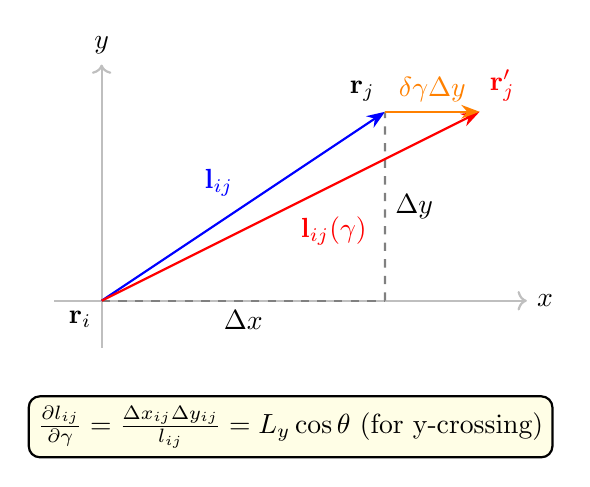
\begin{tikzpicture}[scale=3, thick]
    \coordinate (A) at (0,0);
    \coordinate (B) at (1.2, 0.8);
    \coordinate (Bprime) at (1.6, 0.8);
    
    \draw[->, gray!50] (-0.2,0) -- (1.8,0) node[right, black] {$x$};
    \draw[->, gray!50] (0,-0.2) -- (0,1.0) node[above, black] {$y$};
    
    \draw[blue, -Stealth] (A) -- (B) node[midway, above left] {$\vb{l}_{ij}$};
    \draw[dashed, gray] (1.2, 0) -- (B) node[midway, right, black] {$\Delta y$};
    \draw[dashed, gray] (A) -- (1.2, 0) node[midway, below, black] {$\Delta x$};
    
    \draw[red, -Stealth] (A) -- (Bprime) node[midway, below right] {$\vb{l}_{ij}(\gamma)$};
    \draw[orange, -Stealth] (B) -- (Bprime) node[midway, above] {$\delta \gamma \Delta y$};
    
    \node[below left] at (A) {$\vb{r}_i$};
    \node[above left] at (B) {$\vb{r}_j$};
    \node[above right, red] at (Bprime) {$\vb{r}_j'$};
    
    \node[draw, fill=yellow!10, rounded corners, anchor=north] at (0.8, -0.4) 
        {$\pdv{l_{ij}}{\gamma} = \frac{\Delta x_{ij} \Delta y_{ij}}{l_{ij}} = L_y \cos\theta \text{ (for y-crossing)}$};
\end{tikzpicture}
\end{center}

\subsection{Lees-Edwards Unwrapping \& Area Derivative}
This diagram illustrates why $\pdv{A}{\gamma} \neq 0$ under LEBC. As the box shears, the "unwrapped" ghost cell is shifted horizontally by $\gamma L_y$. For a cell crossing the boundary, this shift changes the shoelace-calculated area if only internal coordinates are tracked.
\begin{center}
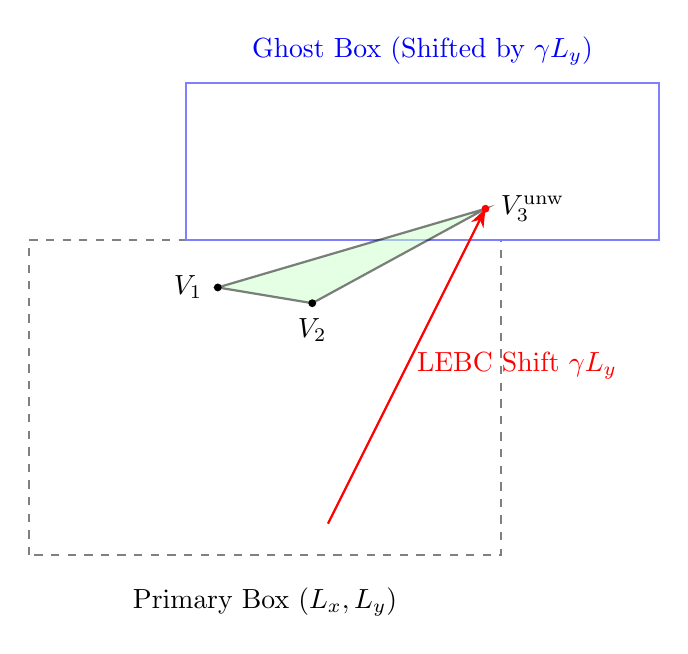
\begin{tikzpicture}[scale=2, thick]
    \draw[dashed, gray] (0,0) rectangle (3,2);
    \node at (1.5,-0.3) {Primary Box ($L_x, L_y$)};
    
    \begin{scope}[shift={(1.0, 2)}] 
        \draw[blue!50] (0,0) rectangle (3,1);
        \node[blue] at (1.5, 1.2) {Ghost Box (Shifted by $\gamma L_y$)};
    \end{scope}

    \coordinate (V1) at (1.2, 1.7);
    \coordinate (V2) at (1.8, 1.6);
    \coordinate (V3wrapped) at (1.9, 0.2);
    \coordinate (V3unwrapped) at (1.9+1.0, 2.2);

    \filldraw[fill=green!20, opacity=0.5] (V1) -- (V2) -- (V3unwrapped) -- cycle;
    \draw[red, -Stealth] (V3wrapped) -- (V3unwrapped) node[midway, right] {LEBC Shift $\gamma L_y$};
    
    \node[circle, fill=black, inner sep=1pt, label=left:$V_1$] at (V1) {};
    \node[circle, fill=black, inner sep=1pt, label=below:$V_2$] at (V2) {};
    \node[circle, fill=red, inner sep=1pt, label=right:$V_3^{\text{unw}}$] at (V3unwrapped) {};
\end{tikzpicture}
\end{center}

\end{document}
